\documentclass[9pt,twocolumn]{article}
\usepackage[a4paper, total={7in, 10in}]{geometry}
\usepackage[utf8]{inputenc}
\usepackage[brazil]{babel}
\usepackage{graphicx}
\usepackage{listings}

%%%%%%%%%%%%%%%%%%%%%%%%%%%%%%%%%%%%%%%%%%%%%%%%%%%%
% C O N F I G U R A Ç Õ E S  D O S   C Ó D I G O S %
%%%%%%%%%%%%%%%%%%%%%%%%%%%%%%%%%%%%%%%%%%%%%%%%%%%%

\lstset{
	numbers=left,
	stepnumber=1,
	firstnumber=1,
	numberstyle=\tiny,
	extendedchars=true,
	breaklines=true,
	frame=single,
	showstringspaces=false,
	xleftmargin=2.5em,
	framexleftmargin=2em,
	basicstyle=\scriptsize,
}

\renewcommand{\lstlistingname}{Código}
\renewcommand{\lstlistlistingname}{Lista de Códigos}

\begin{document}

\section{Representação}

Esta atividade laboratorial tem como objetivo a investigação exploratória de um algorítmo para a classificação de imagens. As imagens analisadas são representações manuscritas de dígitos de 10 categorias diferentes, que representam os número decimais $0,1,2,3,4,5,6,7,8,9$. A figura \ref{fig:image_1_digits} demonstra alguns exemplos das imagens que devem ser classificadas.

\begin{figure}[!htb]
  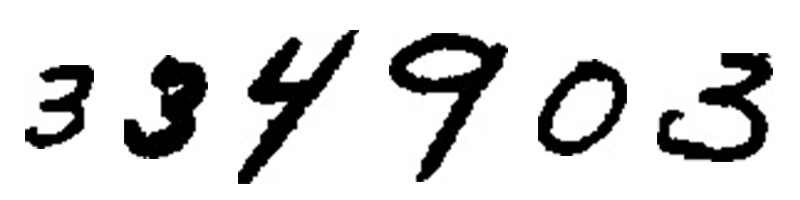
\includegraphics[width=\linewidth]{images/image_1_digits.jpg}
  \caption{Dígitos a serem classificados}
  \label{fig:image_1_digits}
\end{figure}

Além das figuras, um arquivo de texto rotula cada uma das imagens, classificando-a em alguma categoria.

A atividade se iniciou com base na implementação do programa \textit{digits.py} que extrai uma representação bem simples de cada uma das imagens. Para cada imagem, se gera uma nova imagem no tamanho de $10 x 20$. E para cada pixel verifica-se o valor de intensidade do pixel e se esse valor for maior que $128$, a característica é igual a $1$, caso contrário $0$.

Neste ponto, notou-se a possibilidade da primeira exploração. Além do tamanho inicial proposto, uma adaptação no algorítmo realizou uma análise em toda a base de imagens, obtendo outras dimensões para verificação. As estratégias adotadas foram:

\begin{enumerate}
  \item Obter a média entre todas alturas e larguras;
  \item Obter a mediana entre todas alturas e larguras;
  \item Obter os valores máximos entre alturas e larguras;
\end{enumerate}

Após análise dos resultados, notou-se que a média e a media possuam resultados muitos similares, por isso, optou-se apenas pela utilização da mediana. A Tabela \ref{tab:estrategias_representacao} mostra as coleções utilizadas nos experimentos. Além da médiana (med\_x, med\_y) e dos maiores valores(max\_x e max\_y) também foram considerados empiramente os valores de $x,y$ como $[20,40]$ e $[30,60]$.

\begin{table*}[t]
  \centering
  \begin{tabular}{|c|c|c|c|c|c|}
  \hline
  \textbf{X\_Source} & \textbf{Y\_Source} & \textbf{X} & \textbf{Y} & \textbf{File Size} & \textbf{Execution Time (s)} \\ \hline
  10                 & 20                 & 10         & 20         & 2180534            & 1.69                    \\ \hline
  20                 & 40                 & 20         & 40         & 9377970            & 5.44                    \\ \hline
  30                 & 60                 & 30         & 60         & 22978779           & 12.25                   \\ \hline
  med\_x             & med\_y             & 46         & 36         & 20962221           & 11.23                   \\ \hline
  max\_x             & max\_y             & 81         & 99         & 110050116          & 52.76                   \\ \hline
  \end{tabular}
  \caption{Estratégias de representação}
  \label{tab:estrategias_representacao}
\end{table*}

Para automatização da geração das representações, adaptações no código foram realizada para que fosse possível utilizar como entrada um arquivo do tipo JSON demonstrado no Código \ref{code:json_representacao}:

\begin{lstlisting}[caption={JSON para representações},captionpos=b,frame=single,label={code:json_representacao}]
[
  {
    "data": "features_10_20",
    "x": 10,
    "y": 20
  },
  ...
]
\end{lstlisting}

Neste json, \textit{data} é o nome da coleção de representações, $x$ e $y$ podem ser valores fixos ou terem os valores para obtenção dinâmica de: avg\_x, avg\_y, med\_x, med\_y, max\_x, max\_y.

\section{Experimentos}

Assim como na adaptação do primeiro algoritmo, um sistema de entrada JSON possibilitou a variação de combinações para análise de diferentes resultados.

O Código \ref{code:json_experimentos} mostra as opções de entrada para o algorítmo, podendo variar:

\begin{itemize}
  \item O arquivo de representação fonte; as variações testadas foram: [features\_10\_20, features\_20\_40, features\_30\_60, features\_46\_36, features\_81\_99]
  \item Ativar ou desativar a normalização; as variações testadas foram: [0,1]
  \item Alterar o tipo de distância; as variações testadas foram: [eucledian, manhattan]
  \item Alterar o K; as variações testadas foram: [1,3,4,5,6,7,8,9,10,11,12,13]
\end{itemize}

\begin{lstlisting}[caption={JSON para experimentos},captionpos=b,frame=single,label={code:json_experimentos}]
[
  {
    "data": "features_10_20",
    "normalized": 0,
    "distance": "euclidean",
    "k": 1
  },
  ...
]
\end{lstlisting}

\section{Resultados}

Foram realizados 240 execuções para as variações listadas anteriormente. Os 20 melhores resultados de ordenados por acurácia e F1Score estão detalhados na Tabela \ref{tab:resultados}.

Pode-se observar que os melhores resultados foram obtidos a partir das representações que consideraram as maiores alturas e larguras das imagens (81x99). Isso pode ter acontecido pois, no momento em que se realiza a compressão das imagens, características podem ser perdidas. O melhor resultado teve a Acurácia de $0,927$ e o F1Score de $0,928$ demorando $962$ segundos para execução completa.

Na sequência, a estratégia de obter as médias das alturas e larguras também apresentaram resultado significativo (imagens 46x36), mas ficaram empatadas com a estratégia empírica que utiliza imagens 20x40. O destaque aqui é para o tempo de execução. Com a \textit{features\_20\_40} conseguiu-se uma Acurácia de $0,925$ e o F1Score de $0,926$ demorando apenas $43$ segundos para execução completa.

As normalizações não parecem fazer muita diferença nos resultados pois eles se encontram bem distribuídos.

Em geral a alteração da estratégia de medição das distâncias (euclidean e manhattan) não influenciaram em uma melhoria da Acurácia ou do F1Score. O que se pode notar, foi que nos testes executados a estratégia manhattan impacta negativamente no tempo de execução.

Quanto ao $K$ os melhores resultados foram obtidos com $K=1$, seguido de $K=3$ e $K=5$.

\begin{table*}[t]
  \centering
  \begin{tabular}{|c|c|c|c|c|c|c|}
  \hline
  \textbf{Experiment} & \textbf{Normalized} & \textbf{Distance} & \textbf{K} & \textbf{Accuracy} & \textbf{F1Score} & \textbf{Execution Time (s)} \\ \hline
  features\_81\_99    & 0                   & euclidean         & 1          & 0,927             & 0,928            & 962                     \\ \hline
  features\_81\_99    & 0                   & manhattan         & 1          & 0,927             & 0,928            & 1.386                   \\ \hline
  features\_81\_99    & 1                   & euclidean         & 1          & 0,927             & 0,928            & 1.772                   \\ \hline
  features\_81\_99    & 1                   & manhattan         & 1          & 0,927             & 0,928            & 2.495                   \\ \hline
  features\_20\_40    & 0                   & euclidean         & 1          & 0,925             & 0,926            & 43                      \\ \hline
  features\_20\_40    & 0                   & manhattan         & 1          & 0,925             & 0,926            & 86                      \\ \hline
  features\_20\_40    & 1                   & euclidean         & 1          & 0,925             & 0,926            & 127                     \\ \hline
  features\_20\_40    & 1                   & manhattan         & 1          & 0,925             & 0,926            & 170                     \\ \hline
  features\_46\_36    & 0                   & euclidean         & 1          & 0,925             & 0,926            & 597                     \\ \hline
  features\_46\_36    & 0                   & manhattan         & 1          & 0,925             & 0,926            & 686                     \\ \hline
  features\_46\_36    & 1                   & euclidean         & 1          & 0,925             & 0,926            & 771                     \\ \hline
  features\_46\_36    & 1                   & manhattan         & 1          & 0,925             & 0,926            & 859                     \\ \hline
  features\_30\_60    & 0                   & euclidean         & 1          & 0,924             & 0,924            & 214                     \\ \hline
  features\_30\_60    & 0                   & manhattan         & 1          & 0,924             & 0,924            & 314                     \\ \hline
  features\_30\_60    & 1                   & euclidean         & 1          & 0,924             & 0,924            & 406                     \\ \hline
  features\_30\_60    & 1                   & manhattan         & 1          & 0,924             & 0,924            & 504                     \\ \hline
  features\_20\_40    & 0                   & euclidean         & 3          & 0,920             & 0,921            & 46                      \\ \hline
  features\_20\_40    & 0                   & manhattan         & 3          & 0,920             & 0,921            & 89                      \\ \hline
  features\_20\_40    & 1                   & euclidean         & 3          & 0,920             & 0,921            & 131                     \\ \hline
  features\_20\_40    & 1                   & manhattan         & 3          & 0,920             & 0,921            & 173                     \\ \hline
  \end{tabular}
  \caption{Resultados}
  \label{tab:resultados}
\end{table*}

\section{Código Fonte}

Os códigos preparados podem ser analisados através do repositório: https://github.com/diogocezar/machine-learning/tree/master/lab1/src

\end{document}